\chapter{Analyse}

I dette kapitel vil vi gennemgå kravspecifikation til programmet, samt optegne og forklare forskellige modeller.


\section{Kravspecifikation}

\begin{enumerate}
    \item Spilleren og hans pengebeholdning skal kunne bruges i andre spil.
    \item Spilleren skal ikke have mulighed for at slå 1 med to terninger.
    \item Det skal være let at skifte til andre terninger.
    \item Spillet skal kunne let oversættes til andre sprog
    \item Det skal være muligt at kunne arbejde videre på systemet samt følge hvordan
    udviklingen er foregået.
\end{enumerate}

\section{Interessentanalyse}

\begin{center}
    \begin{tabular}{ | l | p{13cm} |}
    \hline
    \textbf{Interresent} & \textbf{Interesse / Mål} \\ \hline
    Spiller/-e & Kunne styre et system, der styrer et spil mellem 2 personer, 
    hvor i der kastes med et raflebæger med to terninger i og ser resultatet med det samme.\\ \hline
    \hline
    \end{tabular}
\end{center}

\section{Use cases}

\begin{table}[H]
    \begin{center}
        \begin{tabular}{ | p{15cm} |}
            \hline
            \textbf{Use case:} PlayGame \\ \hline
            \textbf{ID:} 1 \\ \hline
            \textbf{Brief description} Spiller/-e skal kunne spille spil/Game (starte spillet) og slå med terningen     \\ \hline
            \textbf{Primary actors:} Spiller/-e \\ \hline
            \textbf{Secondary actors:} Ingen. \\ \hline
            \textbf{Preconditions:} Ingen.     \\ \hline
            \textbf{Main flow:}
            \begin{enumerate}
                \item \textbf{Spiller 1 indtaster navn}
                \item \textbf{Spiller 2 indtaster navn}
                \item \textbf{Spiller 1 indtaster 'roll' for at slå med terningen}
                \item \textbf{Spiller 2 indtaster 'roll' for at slå med terningen}
                \item \textbf{Opnås 40 point, og to ens terninger slås, stoppes spillet}    
            \end{enumerate} \\ \hline
            \textbf{Postconditions:} Ingen.\\ \hline
            \textbf{Alternative flow:}
            \\- Ekstra ture gives ved, at slå to ens terninger
            \\- Slås to ens, med 1’ere bliver spillerens score nulstillet
            \\- Spil afsluttes, hvis der bliver slået to 6’ere, med den forudsætning, at to 6’ere blev slået i den forrige runde  \\ \hline
            \hline
        \end{tabular}
        \caption{Use case 1}
        \label{usecase:1}
    \end{center}
\end{table}

\section{Domænemodel}

Der er til projektet udarbejdet en domænemodel for at klarlægge projektets domæne.
Det ses her (figur \ref{fig:domaenemodel}, at spillet består af forskellige elementer som hver har deres forbindelse.
Hele domænet er omfattet af et spil (Game) som består af sprog (Language), terninger (Dice), spillere (Player) og en pengebeholdning (Stash).

\begin{figure}[H]
    \begin{center}
        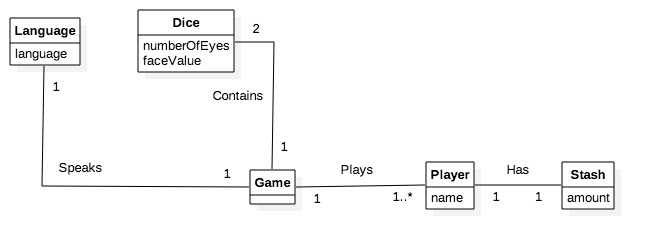
\includegraphics[width=15cm]{graphics/Domainmodel.png}
        \caption{Domænemodel over spillet}
        \label{fig:domaenemodel}
    \end{center}
\end{figure}